\documentclass{article}
\usepackage[utf8]{inputenc}
\usepackage{hyperref}
\usepackage{amsmath}
\usepackage{amsfonts}
\usepackage{graphicx}
\usepackage{physics}

\title{SPhO Ten Year Series (TYS) with Solutions: 2017 Solutions}
\author{
    Solutions available on Victoris\\
    \texttt{victoris.org}
    % new collaborators add your name and contact here!
}

\date{\today}

\begin{document}
\maketitle


\section{2017}
\subsection{Question 1}
1. A planet is in a circular orbit about a massive star of mass $M$. The star undergoes a spherically symmetric explosion where its outer envelope is ejected to a distance well beyond that of the planet's orbit. The remnant of the star has mass $M^{\prime}$ which is still much greater than the mass of the planet. Find the eccentricity of the new orbit of the planet. Assume that the mass loss is instantaneous and that the planet itself is unaffected by the explosion. [10]

\subsection{Solution 1}
Let $R$ and $R'$ be the perihelion and aphelion of the new orbit. Let $v$ and $v'$ be the corresponding velocities. Conservation of angular momentum and energy gives

\begin{align}
    mvR &= mv' R'\\
    \frac{1}{2}mv^2-\frac{GM'm}{R} &= \frac{1}{2}mv'^2-\frac{GM'm}{R'} \\
    v^2(1+R/R') &= \frac{2GM'}{R}
\end{align}

Before the explosion, equating centripetal force to gravitational force gives
\[mv^2/R=GMm/R^2\]

Combining everything
\[1+\frac{R}{R'} = \frac{2M'}{M}\]

The eccentricity can be obtained from
\begin{align}
    \epsilon a &= a-R \\
    \epsilon \left(\frac{R+R'}{2} \right) &= \frac{R+R'}{2} - R\\
    \epsilon &= \frac{M}{M'} - 1
\end{align}

\pagebreak

\subsection{Question 2}
2. Fermat's principle of least time states that the path taken between two points by a ray of light is the path that can be traversed in the least time (which implies stationary optical path length with respect to variations in the path). \\
a) Sketch the path of a light ray travelling from point A to point B as labelled in the diagram below. [2] \\

\begin{figure}
	\centering
	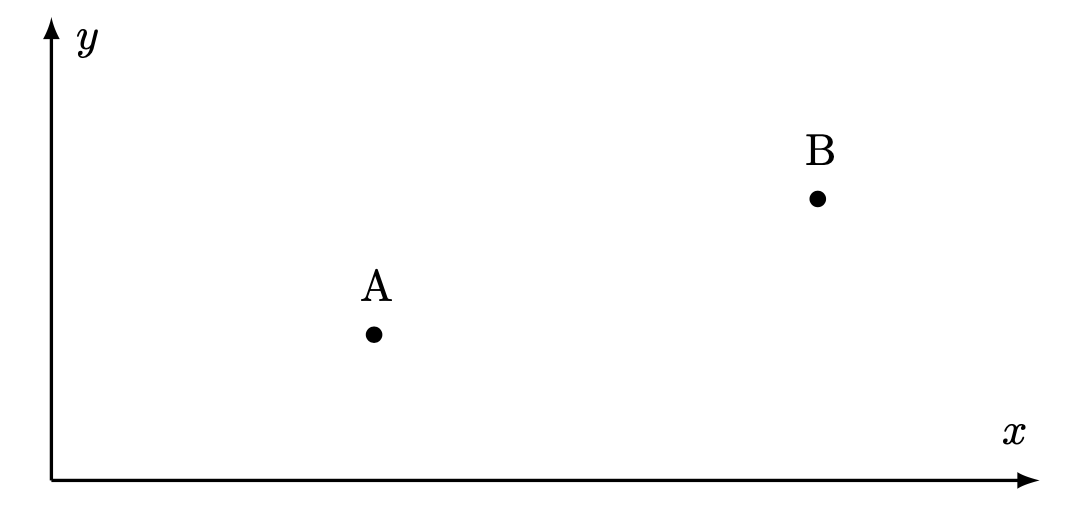
\includegraphics[width=0.5\linewidth]{spho_book_TYS_images/2017q2.png}
	\caption{}
\end{figure}
b) Consider a light ray that also departs from point $\mathrm{A}$, but reflects off the $x$-axis once at a point P before arriving at point B. Applying Fermat's principle to the trajectory APB, determine and sketch the path taken by the light ray. Comment on the angles made by the incident and reflected rays with respect to the surface normal at $P$. [4] \\
c) Now, consider a light ray travelling from point $\mathrm{A}$ to point $\mathrm{B}$ in two media with different indices of refraction, divided sharply by the $y$-axis as shown in the figure below. \\
\begin{figure}
	\centering
	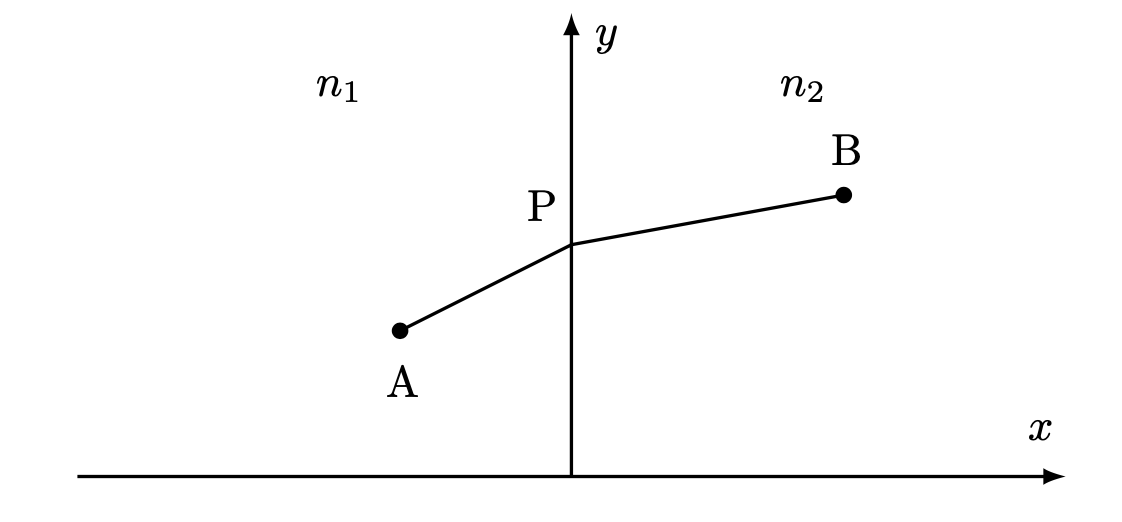
\includegraphics[width=0.5\linewidth]{spho_book_TYS_images/2017q2_2.png}
	\caption{}
\end{figure}
Point $\mathrm{A}$ is in a medium with refractive index $n_{1}$, while point $\mathrm{B}$ is in a medium with refractive index $n_{2}>n_{1}$. The light ray enters the second medium from the first via point P. Applying Fermat's principle to the trajectory APB, determine and sketch the path taken by the light ray. Comment on the angles made by the incident and refracted rays with respect to the surface normal at $\mathrm{P}$. [4]

\subsection{Solution 2}
\subsubsection{Part 2a}
Straight line connecting A and B.

\subsubsection{Part 2b}
Let $x$ be the $x$ coordinate of $P$. Let $\theta_i$ and $\theta_r$ be the angles of incidence and reflection respectively. 

\begin{align}
    l &= \sqrt{(x-x_a)^2+y_a^2} + \sqrt{(x_b-x)^2+y_b^2} \\
    \frac{dl}{dx} &= \frac{x-x_a}{(x-x_a)^2+y_a^2} - \frac{x_b-x}{(x_b-x)^2+y_b^2} = 0 \\
    \cos\theta_i &= \cos\theta_r \Rightarrow \theta_i=\theta_r
\end{align}

\subsubsection{Part 2c}
Let $y$ be the $y$ coordinate of $P$. Let $\theta_1$ ad $\theta_2$ be the angles of incidence and refraction respectively.

\begin{align}
    t &= \frac{\sqrt{x_a^2+(y-y_a)^2}}{c/n_1} + \frac{\sqrt{x_b^2+(y_b-y)^2}}{c/n_2} \\
    \frac{dt}{dy} &= \frac{1}{c}\left( \frac{n_1(y-y_a)}{\sqrt{x_a^2+(y-y_a)^2}} - \frac{n_2(y_b-y)}{\sqrt{x_b^2+(y_b-y)^2}}\right) = 0 \\
    n_1 \sin\theta_1 &= n_2 \sin\theta_2
\end{align}

\pagebreak
\subsection{Question 3}
3. The chlorine radioisotope ${ }^{36} \mathrm{Cl}$ decays to ${ }^{36} \mathrm{Ar}$ with $98.1 \%$ probability and ${ }^{36} \mathrm{~S}$ with $1.9 \%$ probability. In a sample of old groundwater from a cave, the masses of ${ }^{36} \mathrm{Cl}$ and ${ }^{36} \mathrm{~S}$ were measured to be $20 \mu \mathrm{g}$ and $0.36 \mu \mathrm{g}$ respectively. The age of the sample was deduced to be $2.9 \times 10^{5}$ years old from the time of measurement. Calculate the half-life of ${ }^{36} \mathrm{Cl}$.

\subsection{Solution 3}
\begin{align}
    N_{Cl} &= N_{Cl, 0} e^{-\lambda t}, \lambda = \frac{\ln 2}{t_{1/2, Cl}}  \\
    N_S &= \int_0^t \frac{dN_s}{dt} \dd{t} = \int_0^t -0.019 \frac{dN_{Cl}}{dt} \dd{t} = 0.019 N_{Cl} (1-e^{-\lambda t} \\
    \frac{m_{Cl}}{m_S} &= \frac{N_{Cl}}{N_S} = \frac{20}{0.36} = \frac{e^{-\lambda t}}{0.019(1-e^{-\lambda t})} \\
    t_{1/2, Cl} &= \frac{\ln 2}{\lambda} = 3.0\times10^5 \mathrm{years}
\end{align}

In the last step, $\lambda$ can be deduced from the known value of $t$. 

\pagebreak

\subsection{Question 4}
4. An infinite ladder network of capacitors is connected to an $\mathrm{AC}$ voltage supply of $220 \mathrm{~V}$ and $50 \mathrm{~Hz}$ as shown below.
\begin{figure}
	\centering
	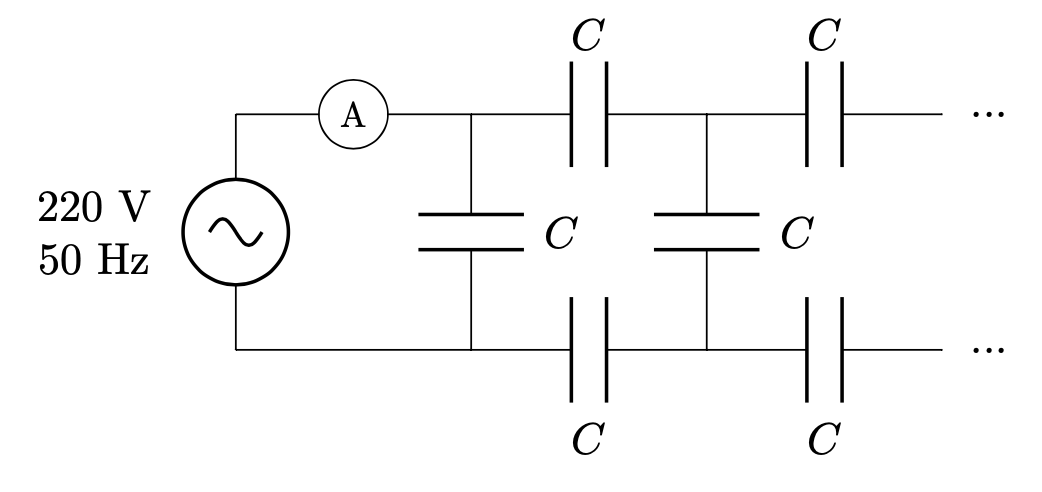
\includegraphics[width=0.5\linewidth]{spho_book_TYS_images/2017q4.png}
	\caption{}
\end{figure}
The capacitance of each capacitor is $1 \mu \mathrm{F}$. Find the current through the ideal $\mathrm{AC}$ ammeter to three significant figures.

\subsection{Solution 4}
The impedance of a capacitor with capacitance $C$ is $Z_C = \frac{1}{i\omega C}$. Let $Z$ be the effective impedance. 
\begin{align}
    \frac{1}{Z} &= \frac{1}{Z_C} + \frac{1}{Z+2Z_C} \\
    Z &= (\sqrt{3}-1) Z_C \\
    I &= \frac{V}{Z} = \frac{V}{(\sqrt{3}-1) Z_C} \\
    &=  \frac{V_0 e^{i\omega t}}{(\sqrt{3}-1)}\cdot i\omega C \\
    \Re(I) &= \frac{V_0 \omega C}{\sqrt{3}-1} \cos(\omega t + \pi/2) \\
    &= 0.0944 \cos (100\pi t + \pi/2)
\end{align}
\pagebreak

\subsection{Question 5}
5. a) An inertial frame $S$ ' travels relative to another inertial frame $S$ with velocity $\beta c$ along the positive $x$-axis. Consider a photon of angular frequency $\omega$ and wavevector $\mathbf{k}$ in $S$. Evaluate the transformations of $\omega$ and $\mathbf{k}$ from $\mathrm{S}$ to $\mathrm{S}$ '. You may quote without proof that $\mathrm{K}^{\mu} \mathrm{X}_{\mu}$ is an invariant quantity, where $\mathrm{K}^{\mu}$ is the 4-wavevector and $\mathrm{X}^{\mu}$ is the 4-displacement. [5] \\
b) A plane mirror moves through vacuum with speed $\beta c$ in the $x$-direction. A beam of light with angular frequency $\omega_{i}$ is incident on the mirror at an angle $\theta_{i}$ to the normal as shown in the figure below. 
\begin{figure}
	\centering
	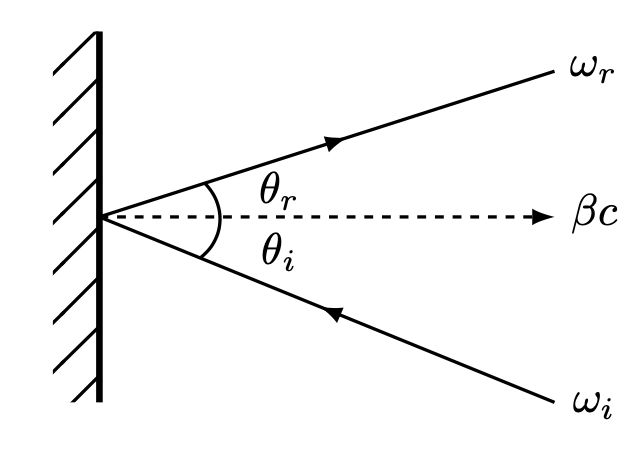
\includegraphics[width=0.5\linewidth]{spho_book_TYS_images/2017q5.png}
	\caption{}
\end{figure}
Determine the angular frequency $\omega_{r}$ and energy $E$ of each reflected photon. [5]

\subsection{Solution 5}

\subsubsection{Part 5a}
The given invariant is 

\begin{align}
    \vec{k'}\cdot\vec{r'} - \omega' t' &= \vec{k} \cdot \vec{r} - \omega t
\end{align}

Applying the Lorentz transformations
\begin{align}
    \gamma k'_x(x-\beta c t) + k'_y y + k'_z z - \gamma \omega' (t-\beta x/c) &= k_x x + k_yy +k_zz-\omega t
\end{align}

Comparing coefficients of $x,y,z,t$,

\begin{align}
    k'_y &= k_y \\
    k'_z &= k_z \\
    k'_x &= \gamma(k_x - \omega\beta/c) \\
    \omega' &= \gamma(\omega - k_x\beta c)
\end{align}

\subsubsection{Part 5b}
Note that the law of reflection holds in the mirror's frame. We will transform the incident 4-wavevector from the lab frame to the mirror frame, apply the law of reflection, and then transform the reflected 4-wavevector from the mirror frame back to the lab frame.

\begin{align}
    k_{xi} &= -k_i\cos\theta_i = -\omega_i \cos\theta_i / c \\
    \omega' &= \gamma(\omega_i - k_{xi}\beta c) = \gamma \omega_i (1+\beta \cos\theta_i) \\
    k'_{xi} &= -k' \cos\theta' = \gamma(k_{xi}-\omega_i \beta / c) = -\gamma \frac{\omega_i}{c} (\cos\theta_i + \beta) \\
    \omega' \cos\theta' &= \gamma \omega_i (\cos\theta_i + \beta) \\
    \cos\theta' &= \frac{\cos\theta_i + \beta}{1+\beta\cos\theta_i} \\
    \omega_r &= \gamma(\omega' + k'_x \beta c) \\
    k'_x &= \frac{\omega'}{c}\cos\theta' \\
    \omega_r &= \gamma \omega' (1+\beta \cos\theta') \\
    &= \gamma^2 \omega_i (1+2\beta\cos\theta_i +\beta^2) \\
    E =&= \hbar \omega_r = \hbar \gamma^2 \omega_i (1+2\beta\cos\theta_i +\beta^2)
\end{align}

\pagebreak

\subsection{Question 6}
6. Two identical balloons are inflated to different radii and connected via a thin tube. Contrary to conventional intuition, the smaller balloon deflates and the larger balloon inflates, instead of reaching an equal size. To explain this counter-intuitive result, we analyse the pressure-tension relation of stretching rubber. \\
a) The tension in a surface element of a stretched rubber balloon is
$$
F \propto \frac{r}{r_{0}^{2}}\left[1-\left(\frac{r_{0}}{r}\right)^{6}\right]
$$
where $r$ is the radius of the inflated balloon and $r_{0}$ is the original radius of the balloon. The figure below shows the tension acting on the surface element that arises from stretching the rubber, which acts tangential to the balloon.
\begin{figure}
	\centering
	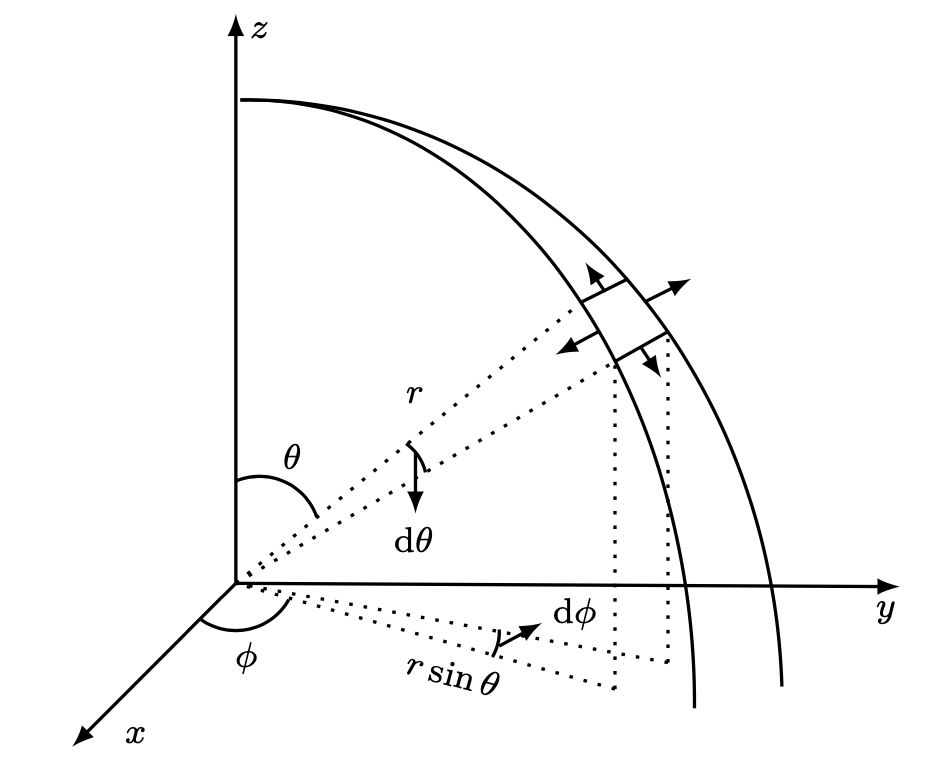
\includegraphics[width=0.5\linewidth]{spho_book_TYS_images/2017q6.png}
	\caption{}
\end{figure}
i) Show that the internal air pressure of the balloon, relative to the atmospheric pressure, is given by
$$
P=\frac{C}{r_{0}^{2} r}\left[1-\left(\frac{r_{0}}{r}\right)^{6}\right]
$$
where $C$ is a constant. [3] \\
ii) Show that the radius of the balloon at which the internal pressure is maximum is $r_{\max }=7^{\frac{1}{6}} r_{0}$. [1] \\
iii) Sketch the pressure-radius graph of the balloon. Label the points $r_{0}$ and $r_{\max }$ on your graph. [2] \\
b) Now, consider two balloons of two different radii connected via a thin tube. Initially, the smaller balloon is at its maximum radius, i.e. it has radius $r_{s_{i}}=7^{\frac{1}{6}} r_{0}$. After air is exchanged and the two balloons reach equilibrium, the final radius of the smaller balloon is $r_{s_{f}}=6^{\frac{1}{6}} r_{0}$. \\
i) Calculate the final radius of the bigger balloon $r_{b_{f}}$ at equilibrium as a multiple $r_{0}$ to three significant figures. You may use numerical methods to obtain your answer. [2] \\
ii) Calculate the initial radius of the bigger balloon $r_{b_{i}}$ as a multiple $r_{0}$ to three significant figures. You may use numerical methods to obtain your answer. You may use numerical methods to obtain your answer. [3] \\
iii) Suppose that the tube has cross-sectional area $A$, the average mass of an air molecule is $m$, and the experiment is conducted in a controlled environment of temperature $T$. Assuming that the tube is long and thin enough for the flow rate to be characterised by the r.m.s. speed of the particles constrained to a single dimension, show that the time taken for the two balloons to reach equilibrium is
$$
t \simeq \frac{16 \pi}{3 A} \sqrt{\frac{m}{k_{B} T}} \int_{r_{b_{i}}}^{r_{b_{f}}} \mathrm{~d} r_{b} \frac{r_{b}\left[1-2\left(\frac{r_{0}}{r_{b}}\right)^{6}\right]}{\frac{1}{r_{s}}\left[1-\left(\frac{r_{0}}{r_{s}}\right)^{6}\right]-\frac{1}{r_{b}}\left[1-\left(\frac{r_{0}}{r_{b}}\right)^{6}\right]}
$$
where $r_{s}$ and $r_{b}$ are the radii of the smaller and bigger balloons at a given instant respectively. [4]

\subsection{Solution 6}
\subsubsection{Part 6ai}
Consider a hemisphere of the balloon. The force due to surface tension equals the force due to pressure. 
\begin{align}
    Fr &= P\pi r^2 \\
    P &\propto F/r \\
    P &=\frac{C}{r_{0}^{2} r}\left[1-\left(\frac{r_{0}}{r}\right)^{6}\right]
\end{align}

\subsubsection{Part 6aii}
Maximum pressure is attained when $\frac{dP}{dr}=0$.
\begin{align}
    \frac{dP}{dr} &= \frac{C}{r_0^2}\left(-\frac{1}{r^2} + \frac{7r_0^6}{r^8}\right) = 0 \\
    r_{\max} &= 7^{1/6} r_0
\end{align}

\subsubsection{Part 6aiii}
This is left as an exercise for the reader. Any graphing tool will suffice.

\subsubsection{Part 6bi}
\begin{align}
    P_f &= P(r_{sf}) = \frac{5C}{6^{7/6}r_0^3} \\
    \frac{5C}{6^{7/6}r_0^3}  &= \frac{C}{r_0^2 r}\left(1-\left(\frac{r_0}{r}\right)^6\right) \\
    r &= 6^{1/6} r_0 \\
    r_{bf} &= 1.42 r_0
\end{align}

\subsubsection{Part 6bii}
The total number of air molecules is constant
\[N_{bi} = N_{si} = N_{bf} + N_{sf}\]

Using $PV = NkT, T=\mathrm{const}$,

\[P_{bi}V_{bi} + P_{si}V_{si} = P_{bf}V_{bf}+ P_{sf}V_{sf} \]

Because $P_{bf} = P_{sf} = P_f$ and $P_{si}=P_{\max}$
\[P_{bi}V_{bi}+P_{\max}V_{si} = P_f(V_{bf} + V_{sf})\]

Substituting the expressions and solving,
\[r_{bi} = 1.387 r_0\]

\subsubsection{Part 6biii}
The number of molecules going through the tube is
\[\dd{N} = \frac{1}{2} nvA\dd{t}\]

The factor of 1/2 accounts for the fact that only half of the molecules are going towards the other balloon.

\begin{align}
    \frac{dN}{dt} = \frac{1}{2} nvA = \frac{NA}{2V} \sqrt{\frac{kT}{m}} = \frac{PA}{2kT} \sqrt{\frac{kT}{m}} 
\end{align}

Summing the contributions - outflow of big balloon and inflow from small balloon,
\begin{align}
    \frac{dN_b}{dt} &= \frac{P_sA}{2kT} \sqrt{\frac{kT}{m}} - \frac{P_bA}{2kT} \sqrt{\frac{kT}{m}} \\
    &= \frac{AC}{2kT r_0^2} \sqrt{\frac{kT}{m}} \left( 
        \frac{1}{r_s} \left( 1 - \left(\frac{r_0}{r_s}\right)^6 \right) -
        \frac{1}{r_b} \left( 1 - \left(\frac{r_0}{r_b}\right)^6 \right)
    \right)
\end{align}

We also know from the ideal gas equation that
\begin{align}
    P_b V_b &= N_b kT \\
    N_b &= \frac{4\pi C}{3kTr_0^2} \left(r_b^2 - \frac{r_0^6}{r_b^4} \right) \\
    \frac{dN_b}{dt} &= \frac{8\pi C r_b}{3kTr_0^2} \left(1+2\left(\frac{r_0}{r_b}\right)^6\right) \frac{dr_b}{dt}
\end{align}

Comparing the two expressions, we have
\begin{multline}
 \frac{AC}{2kT r_0^2} \sqrt{\frac{kT}{m}} \left(         \frac{1}{r_s} \left( 1 - \left(\frac{r_0}{r_s}\right)^6 \right) -
        \frac{1}{r_b} \left( 1 - \left(\frac{r_0}{r_b}\right)^6 \right)
    \right) \\
    =\frac{8\pi C r_b}{3kTr_0^2} \left(1+2\left(\frac{r_0}{r_b}\right)^6\right) \frac{dr_b}{dt} 
\end{multline}

This simplifies to
\[\dd{t} = \frac{16 \pi}{3 A} 
\sqrt{\frac{m}{k_{B} T}}
\frac{r_{b}\left[1+2\left(\frac{r_{0}}{r_{b}}\right)^{6}\right]}
{\frac{1}{r_{s}}\left[1-\left(\frac{r_{0}}{r_{s}}\right)^{6}\right]-\frac{1}{r_{b}}\left[1-\left(\frac{r_{0}}{r_{b}}\right)^{6}\right]} 
\dd{r_b}
\]

7. a) Consider a volume $V$ bounded by a closed surface $\partial V$. There exist electrostatic fields $\mathbf{E}_{\text {in }}$ and $\mathbf{E}_{\text {out }}$ inside and outside $V$. Derive the boundary condition
$$
E_{\mathrm{out}}^{\perp}(\mathbf{r})-E_{\mathrm{in}}^{\perp}(\mathbf{r})=\frac{\sigma(\mathbf{r})}{\epsilon_{0}}
$$
where $\mathbf{r}$ is the position vector of any point along $\partial V, E^{\perp}(\mathbf{r})$ is the perpendicular component of $\mathbf{E}(\mathbf{r})$ to the surface at $\mathbf{r}, \sigma(\mathbf{r})$ is the surface charge density at $\mathbf{r}$, and $\epsilon_{0}$ is the permittivity of free space. [4] \\
b) Suppose $V$ is spherical and contains a continuous charge distribution with constant volume charge density $\rho$. Show that if $E_{\text {out }}\left(R^{-}\right)=E_{\text {in }}\left(R^{+}\right)$, then $\sigma$ is zero everywhere along $\partial V$. [5] \\
c) Suppose $V$ is a spherical conductor of radius $R$ and total charge $Q .$ If $V$ is cut into half, what is the repulsive force between the two halves? [6] 

\subsection{Solution 7}
\subsubsection{Part 7a}
Consider a Gaussian pillbox surrounding an area $\dd{A}$ on the surface. Applying Gauss' Law,
\[(E_{out}^+ - E_{in}^+) \dd{A} = \frac{\sigma \dd{A}}{\epsilon_0}\]

Taking the limit $h\rightarrow 0$ (where $h$ is the height of said pillbox), this simplifies to the desired result.
\subsubsection{Part 7b}
This follows from the result of 7a, combined with spherical symmetry.

\subsubsection{Part 7c} 
As V is a conductor, $E$ is zero inside $V$ (excluding the boundary), and charges are only present on $\partial V$. It is easy to see that $\sigma = Q/4\pi R^2$.

By Gauss' Law, we know the electric field to be
\[E(R+) = \frac{\sigma}{\epsilon_0}, E(R-) = 0\]

We can take $E(R)$ to be the average, $\frac{\sigma}{2\epsilon_0}$ (a rigorous treatment is omitted for the sake of brevity).

The force experienced by an area $\dd{A}$ on the surface is
$\dd{F} = \sigma E(R) \dd{A} = \frac{\sigma^2}{2\epsilon_0} \dd{A}$. So the sphere experiences an electrostatic pressure of $P=\frac{\sigma^2}{2\epsilon_0}$.

The total repulsive force is then the product of the electrostatic pressure with the normal cross sectional area \[F = \frac{\sigma^2 \pi R^2}{2\epsilon_0}\]
\end{document}
